\documentclass[zad,zawodnik,utf8]{sinol}

\title{Skittlesy}
\id{ski}
\author{Maciej Hołubowicz} % Autor zadania
\pagestyle{fancy}
\iomode{stdin}
\konkurs{XIV obóz informatyczny}
\etap{olimpijska}
\day{1}
\date{16.01.2017}
\RAM{8}

\usepackage{graphicx}
 
\begin{document}
\begin{tasktext}%

Marcin ma aż $n$ Skittlesów ułożonych w ciągu. Kolory Skittlesów, które ma Marcin, to czarny albo biały. Marcin przechwalał się Przemkowi, że jest bardzo fajny, bo ma dużo Skittlesów {\it 'i wogule'}. Przemka to wkurza i chce udowodnić Marcinowi, że wcale nie jest taki fajny! Przemek chciałby wybrać ciąg Skittlesów, który nie występuje jako podsłowo w ciągu Skittlesów Marcina i udowodnić mu, że jest w błędzie i nie jest taki fajny, bo nawet nie ma takiego krótkiego ciągu Skittlesów jako podsłowo! Oczywiście Przemek chciałby użyć jak najmniej Skittlesów (bo nie jada takich świństw).

  \section{Wejście}
Pierwszy wiersz wejścia zawiera jedną liczbę całkowitą $n$ ($1 \leq n \le 5 \cdot 10^7$) oznaczającą liczbę Skittlesów posiadanych przez Marcina.
Kolejny wiersz zawiera $n$ zer lub jedynek, oznaczająca kolejne kolory Skittlesów. 1 oznacza czarny kolor a 0 biały.

\begin{center}
Jako że wejście jest duże, zalecamy wczytywać je w ten sposób:\\
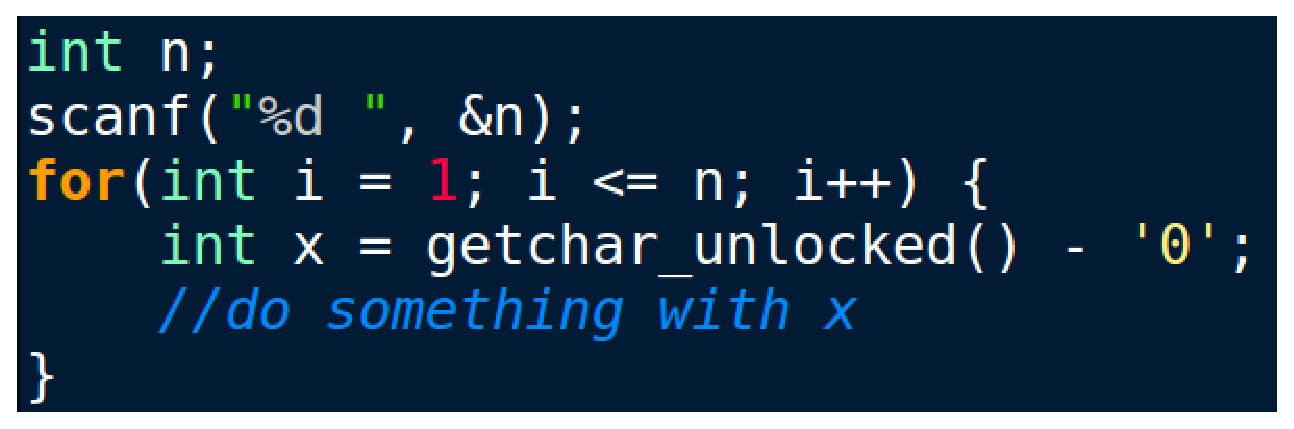
\includegraphics[height=4cm]{rowski.eps}\\
Można też użyć samego $getchar()$, ale jest to trochę wolniejsze.
\end{center}

 \section{Wyjście}
Pierwszy i jedyny wiersz wyjścia powinien zawierać jedną liczbę całkowitą, oznaczającą minimalną długość ciągu zero-jedynkowego, który nie występuje jako podsłowo słowa z wejścia.

\makecompactexample

\end{tasktext}
\end{document}
